\documentclass[12pt]{article}
\usepackage{mathtools, amsmath, amsfonts, amssymb}
\usepackage{hyperref, graphicx, wrapfig, geometry}
\usepackage[makeroom]{cancel}


\newgeometry{margin=2cm}

\title{Microprocessor Systems - Lab report}
\author{Auguste Lalande, Felix Dube, Juan Morency Trudel}
\date{\today}

\begin{document}
\maketitle
\clearpage

\tableofcontents
\clearpage

\section{Abstract}
This project involves measuring the temperature of the STM32F407 processor and displaying the value in celsius on a display. Data are being filtered using a Kalman filter. Lastly, an overheating alarm have been implemented.

\section{Problem Statement}
The temperature of the temperature needs to be monitored in order to avoid over heating it. The user should be able to monitor the temperature in meaningful units, and he should be advised if the processor is overheating.

\section{Theory and Hypothesis}
\subsection{Temperature Sensor}
In order to measeru the temperature of the processor, the internal temperature sensor will be used. It is hard wired to the channel 16 of ADC1 inside the processor.

\subsection{Analog to Digital Converter}
The ADC will be used in polling mode in order to convert the analog value of the temperature sensor to a 12 bits digital value.

\subsection{Systick}
Systick is a process that count the period of the processor clock. It start to a predefinned value and count down to 0. When it reaches to 0, the Systick handler is called. This will be used to set up various timing requirement of the project.

\subsection{General Purpose Input Output}
GPIOs are used in order to for the processor to communicate with external components. 

\subsection{7-Segments Displays}
The 7-segment displays are LED diplay for which the segment can be individually controled to display the appropriate character.

\subsection{LCD Display}
An alternative way of presenting the temperature is to use an LCD display. The display used for the project is an LCD diplay made by sparkfun with part number adm1602k-fsy-ybs/z. The processor comunicate with the display using 2 control bit and an 8 bits data bus. On the display, each character position is an address in memory (memory of the display itself). In order to write something on the disaplay, the character needed to be displayed needs to be saved at the appropriate memory address.


\section{Implementation}
\subsection{Sampling Data}

\subsection{Filtering Data}
\begin{figure}[!htb]
\centering
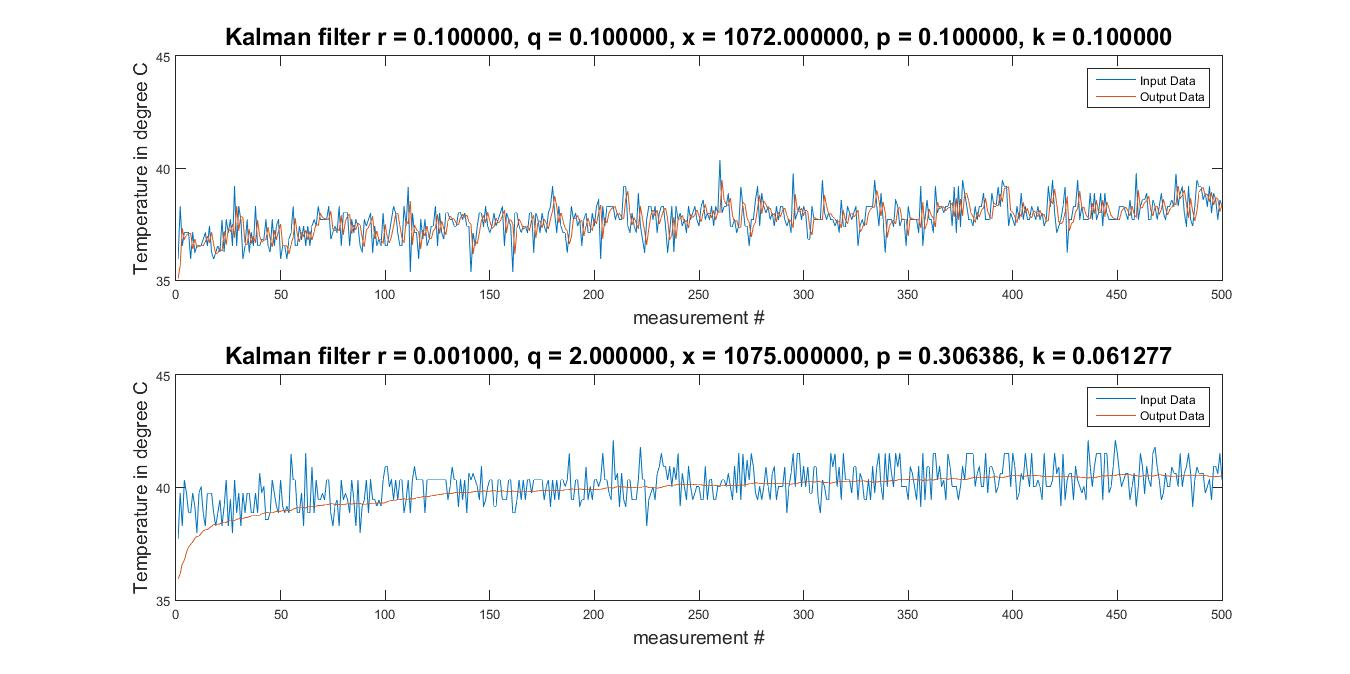
\includegraphics[scale=0.35]{images/kalmanfilter.jpg}
\caption{Filtered Data Compared to Raw Data Before and After Optimising the Kalman Filter Parameters}
\label{fig:kalmanfilter}
\end{figure}

\subsection{Displaying the Data}

\subsection{Overheating Alarm}

\section{Observation}

\section{Conclusion}
\newpage

\section{Appendix}

\end{document}
